% based on https://www.overleaf.com/latex/templates/writing-posters-with-markdown/jtbgmmgqrqmh

\documentclass{beamer}
%% Possible paper sizes: a0, a0b, a1, a2, a3, a4.
%% Possible orientations: portrait, landscape
%% Font sizes can be changed using the scale option.
\usepackage[size=a0,orientation=landscape,scale=0.8]{beamerposter}
\usetheme{Simula-poster}
\usecolortheme{simula}

\usepackage{booktabs}
\usepackage{subfig}
\usepackage{csvsimple}
\usepackage[utf8]{inputenc}
\usepackage[T1]{fontenc}
\usepackage{helvet}
\usepackage[scaled=0.92]{inconsolata}
% \usepackage[libertine]{newtxmath}
\usepackage{natbib}
\renewcommand{\bibfont}{\small}

\newcommand{\texthash}{\#}

%% Load the markdown package
\usepackage[citations,footnotes,definitionLists,hashEnumerators,smartEllipses,tightLists=false,pipeTables,tableCaptions,hybrid]{markdown}
%%begin novalidate
\markdownSetup{rendererPrototypes={
 interblockSeparator = {\par\vspace{1ex}},
 link = {\href{#2}{#1}},
 headingFour = {\begin{block}{#1}},
 horizontalRule = {\end{block}}
},
}
%%end novalidate

\author[]{Vilde Dille Øvreeide and Min Ragan-Kelley}
\institute[simula]{Simula Research Laboratory}

\title{Measuring notebook reproducibility with repo2docker}
% Optional foot image
\footimage{
\includegraphics[width=8cm]{simula-logo.pdf}}

\begin{document}
\begin{frame}[fragile]\centering

\begin{columns}
\begin{column}{0.5\textwidth}

\begin{markdown}{tightLists=false}

#### Motivation


- A large-scale study of notebook reproducibility was published in 2019 [@reproducibility:2019]
- repo2docker is a tool for automatically generating environments from repos, to aid in reproducibility [@binder2]
- we want to evaluate repo2docker's automatic env generation,
  and compare with the study's conclusions
- Study did not evaluate execution of languages other than Python;
  whereas repo2docker can produce environments with Julia, R, etc.
- repo2docker has no mechanism for evaluating success other than `docker build` completing without error


----
\end{markdown}
\end{column}

\begin{column}{.5\textwidth}
\begin{markdown}


#### Caveats

- For evaluating repo2docker, our main interest is in *environment reproducibility*,
  not *code reproducibility*,
  so if all dependencies are met, the goal is achieved.
  But how can we tell if an error is because the environment is wrong,
  or if the notebook itself is in error?
- Relying on data from [@reproducibility:2019] means many repositories have not been updated since 2018.
- **What qualifies as a successfully reproducible repo?**
  We chose the minimum: repo2docker successfully builds an image, and

    - it has notebooks
    - notebooks execute without error

----

\end{markdown}
\end{column}

\end{columns}

\bigskip
{\usebeamercolor[bg]{headline}\hrulefill}
\bigskip

\begin{columns}[T]

%%%% First Column
\begin{column}{.3\textwidth}

\begin{markdown}


#### Process

1. collect repositories to test
    - source 1: queries from previous study [@reproducibility:2019]
    - source 2: Binder Events Archive [@binder-events]
2. build image with repo2docker
3. find notebooks in repo (up to 5)
4. execute notebooks with nbconvert (record results) in repo2docker-built image
5. record results in csv, organized by repository and ref

Steps 2-5 are automated with repo2docker-checker [@repo2dockerchecker],
a thin wrapper around repo2docker that adds execution via nbconvert
and collecting test results and build logs.


----

#### Repository categories

We collected groups of repositories to sample from different sources.

First, we queried the study database for several categories we should expect different kinds of results from,
grouped by classification in the study:


- **Julia** notebooks (not tested previously). We should expect these to install Julia and have some execution success.
- **R** notebooks (not tested previously). We should expect these to install R and have some execution success.
- **Installation failed** (environment specified, could not install). We expect these repos to fail to build during installation.
- **Import error** / ModuleNotFound (likely missing dependency specification). We expect these repos to fail in a similar way to that seen in the study.
- **Success without dependencies** (environment not found by study, run in Anaconda without error). Because repo2docker does not use a full Anaconda environment by default, we expect many of these to fail with ImportErrors, depending on whether the standard library is all that is required.
- **Success with dependencies** (dependencies found by study, may not be found by repo2docker). We expect these to succeed at a rate comparable to the rate at which repo2docker is able to locate the environment specification
- **Success with top-level requirements.txt** (Subset of above where dependencies are specified in a requirements.txt file in the base directory of the repo.) We expect these to succeed.
- **Success with Pipfile** (environment specified by pipfile, execution succeeds). We expect these to succeed.

Critically, this does not assume repos which were written with repo2docker in mind,
testing the "automate existing best practices" goal of repo2docker.

We also used one more source of repos, top repos from the **Binder Events Archive** [@binder-events],
which are known to work with repo2docker and and be popular on the mybinder.org service.
If these repos aren't considered to work, our validation strategy should be re-evaluated.

----

#### Outcomes

There are several possible outcomes,
with several causes,
and several times and ways in which to fail.
Some failures are interesting for the purposes of repo2docker,
others are not:

- **build failure** - repo2docker fails to construct a working image
    + due to partially pinned environment (e.g. pinned numpy not compatible with Python 3.8)
    + due to pre-build dependencies (e.g. apt-get install C libraries)
    + actually invalid requirements (rare!)
    + Failure to detect runtime, e.g. Julia
- **execution failure**
    + **ImportError**
        - environment not specified at all
        - environment insufficiently specified
        - environment specified in a location or format not recognized by repo2docker
    + user input/editing required (e.g. credentials for using an API, or "fill out X before executing"). These are valid notebooks, but cannot be automatically validated.
    + assumption of context (e.g. computational resources, manual setup steps in README)
    + actual bugs in notebooks. These are failures in reproducibility, but not failures for repo2docker to investigate further
- **success** - image is built and notebooks execute without error

----


\end{markdown}

\end{column}

%%%% Second Column
\begin{column}{.4\textwidth}

\begin{block}{Results}

\center
% \setkeys{Gin}{width=.3\linewidth}
\csvautotabular{../data_collection/results.csv}
% ![exampleimage](example-image.jpg "An exemplary image")
% \begin{tabular}{|l|l|l|}
%  \csvnames{myNames}{1=\category,2=\repos,3=\success,4=\build,5=\failure,6=\importerror}
% \hline
% Group & Repos & Success & Build failure & Execution failure & Failed with import error
% \csvreader[myNames]{../data_collection/results.csv}{}%
% {\\\givenname\ \name & \matriculation}%
%  \\\hline
%  \end{tabular}


% | Right | Left | Default | Center |
% |------:|:-----|---------|:------:|
% |  12   |  12  |  12     |   12   |
% | 123   |  123 |   123   |  123   |
% |   1   |    1 |     1   |    1   |

%   : Demonstration of pipe table syntax.

% side-by-side figures
% \begin{figure}%
%     \centering
%     \subfloat[\centering Total counts for success \& failure for each group of repos]{{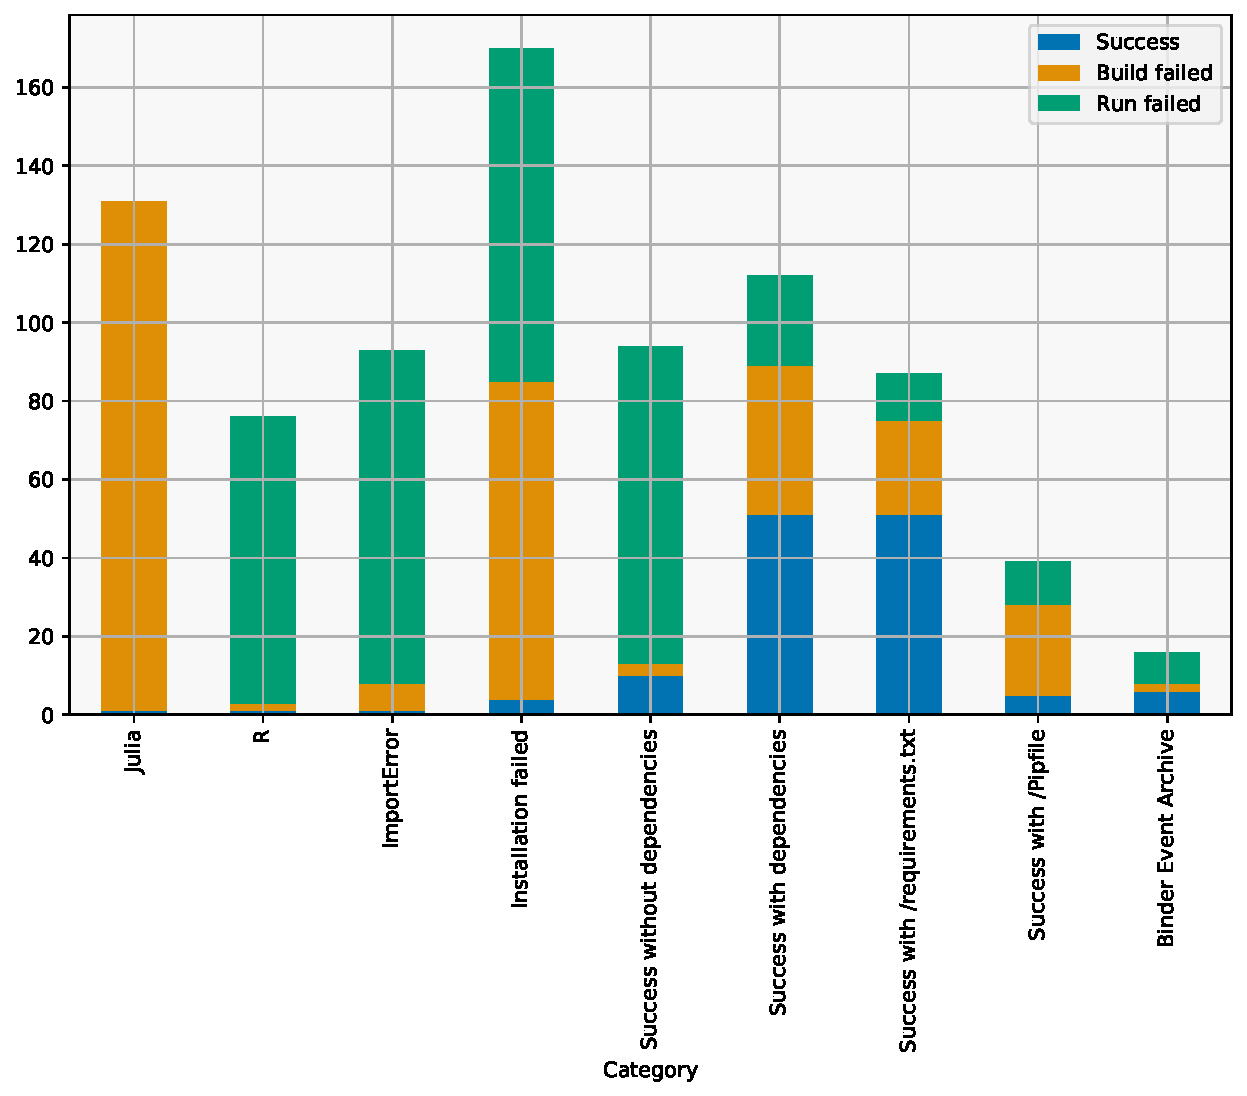
\includegraphics[width=0.4\textwidth]{fig/totals.pdf} }}
%     \qquad
%     \subfloat[\centering Rates for success and failure, separating execution failure due to ImportError]{{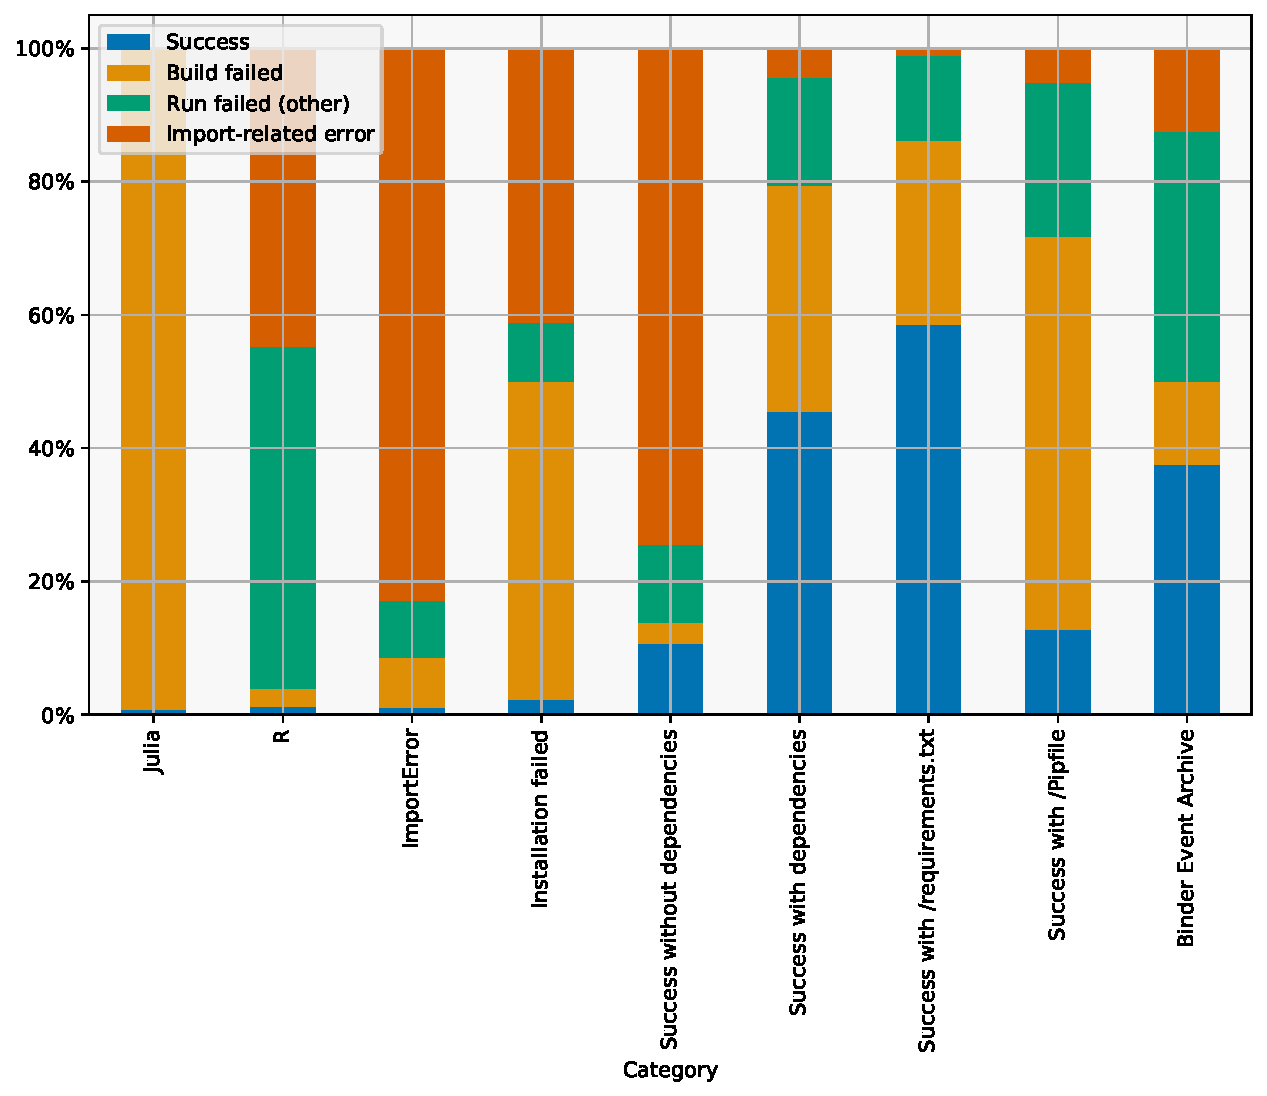
\includegraphics[width=0.4\textwidth]{fig/rates.pdf} }}
%     \caption{Total result counts and relative error rates.}
%     \label{fig:example}
% \end{figure}

\begin{figure}%
    % \centering
    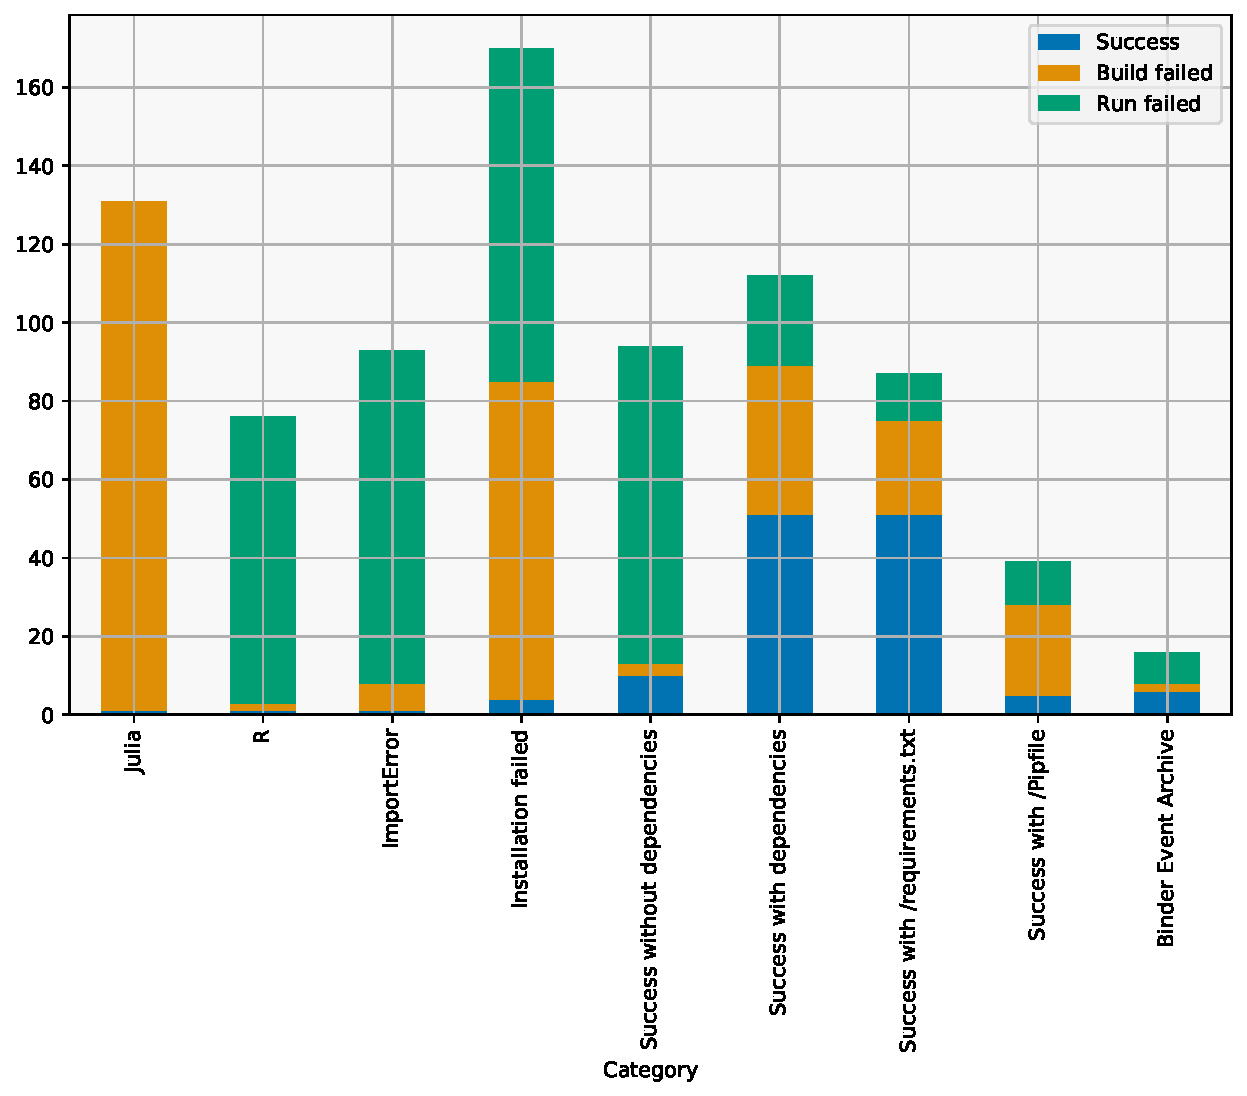
\includegraphics[width=0.6\textwidth]{fig/totals.pdf}
    % \caption{Total counts for success \& failure for each group of repos}
\end{figure}

\begin{figure}%
    % \centering
    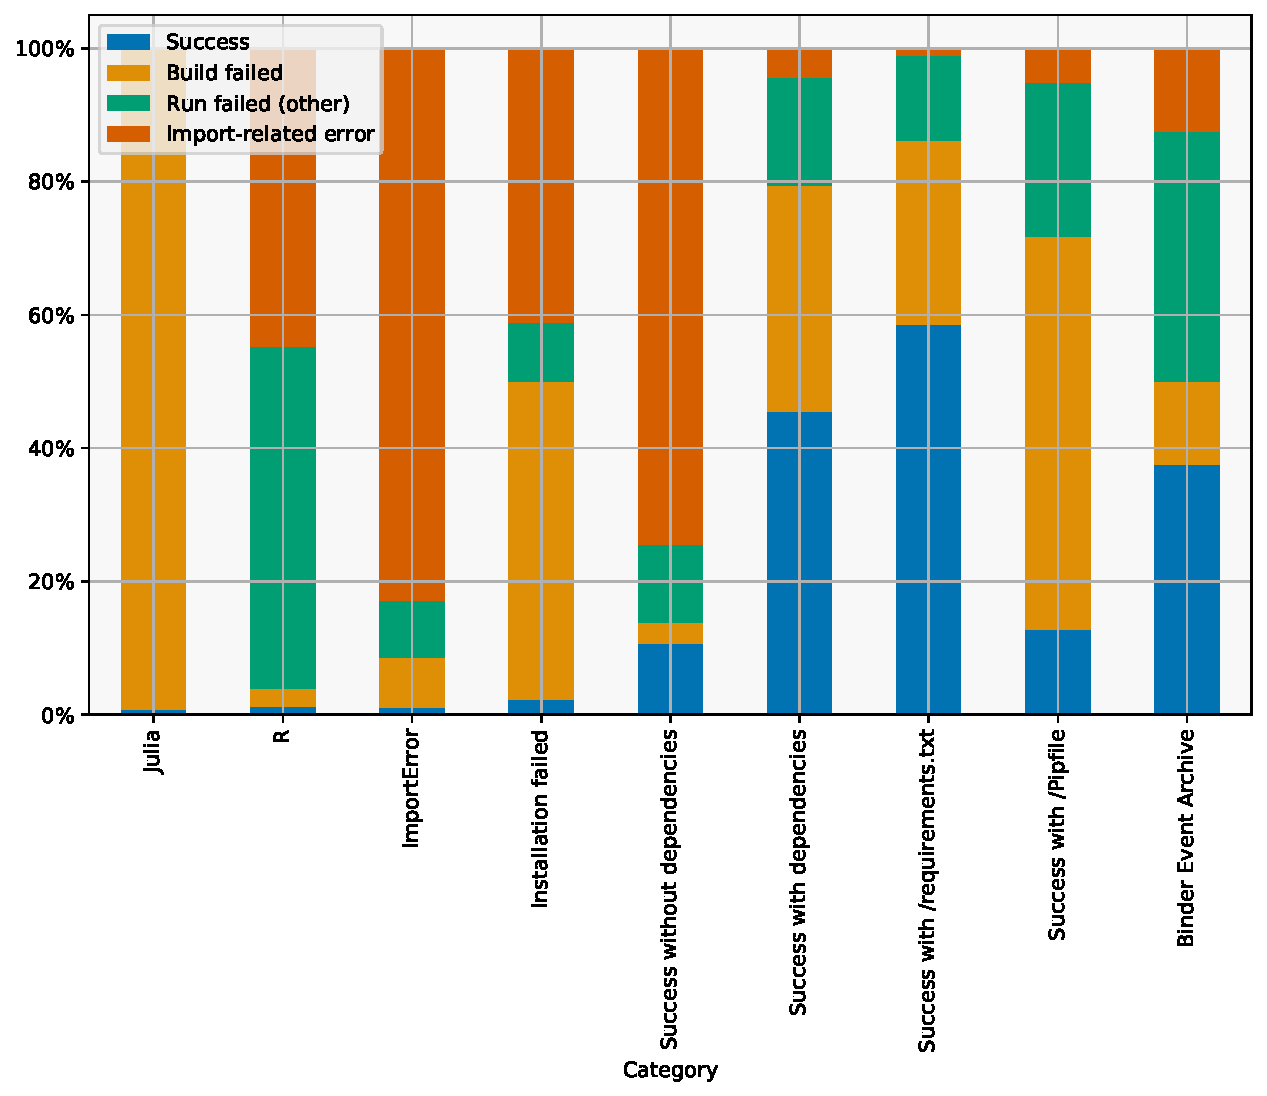
\includegraphics[width=0.6\textwidth]{fig/rates.pdf}
    % \caption{Rates for success and failure, separating execution failure due to ImportError.}
\end{figure}

\end{block}

\begin{markdown}


\end{markdown}


\end{column}

%%%% Second Column
\begin{column}{.3\textwidth}
\begin{markdown}

#### Highlights

Expected results:

- Majority of repositories reported raising **ImportErrors** in [@reproducibility:2019] had same results with repo2docker
- Large fraction of **install failed** repos also failed with a build error, but ~half did not.
  This matches the 54\% rate of successfully executing repos having environment specified in default /requirements.txt location which repo2docker would find.
- **Success without dependencies** has a high rate of ImportError,
  which is expected because this group lacks environment specifications
  found in [@reproducibility:2019] but was executed in an Anaconda environment.
  repo2docker's smaller base environment lacks the common dependencies for most of these repos.
- Success rate with requirements.txt at the default location (where repo2docker will find it) is highest, but still below 60\%.
  Many failures were due to incomplete pinning.



Unexpected results:

- Exactly one Julia repo installed Julia: Binder's own Julia example.
  Repo2docker offered ~no benefit over not testing Julia at all
  for a sample of real repos containing Julia notebooks in 2018.
- R success rate was similarly extremely low, despite installing R more often.
- **Pipfile/Pipfile.lock** success rate is lower than requirements.txt.
  Investigating build logs shows that strictly pinning numpy, etc. is common
  while pinning Python is rare, despite the fact that Pipfiles do support pinning Python itself.
- Many popular repos on Binder don't pass our execution test,
  meaning they may contain notebooks that do not run without modification.
  Does this mean our validation is not particularly useful?

Perhaps the most significant result, in our eyes: **A very common source of build failure is strictly pinning dependencies numpy or pandas and not pinning Python**. Due to the age of most tested repos,
  this means many instances of \texttt{numpy==1.14.1} which cannot be installed
  with Python 3.8, the default Python for repo2docker.


----


#### Conclusions

- Open data publication in [@reproducibility:2019] greatly facilitates follow-up studies!
- A large fraction of build failures were due to pinning packages (most often numpy or pandas)
  but not Python, because there is no community standard for pinning Python (conda, Pipfile insufficiently common, often lack Python itself)
- repo2docker success rate could be greatly improved if we looked at more of the repo to determine runtime language and/or version:
    + last repository commit date could pick older Python by default (not at all intrusive)
    + notebook \texttt{language info} metadata includes runtime and version (more expensive to evaluate)
- repo2docker does not implement best practices adopted in R and Julia communities
    + big caveat for Julia: most repos tested were older than the advent of the new \texttt{project.toml}

----

#### Future work

- Test repo2docker with different strategies for picking runtimes / versions
- Evaluate more repos, our sample size was small
- Plugin check to Binder for more thorough evaluation of success on build
- Engage with R / Julia community to investigate standards for specifying environments.
  **Is repo2docker missing something, or do these communities not have widely used environment standards?** Specifically, evaluate adoption of recently implemented ``project.toml`` specification.

----

#### Bibliography

\bibliographystyle{unsrtnat}
\bibliography{refs}

----

\end{markdown}
\end{column}
\end{columns}

\end{frame}


\end{document}
